\documentclass[11pt]{report}

\RequirePackage[banglamainfont=Kalpurush, banglattfont=SiyamRupali, feature=2]{latexbangla_exp}

\usepackage{ragged2e}
\usepackage{blindtext}

\usepackage{epigraph}
\usepackage{amsmath,amsfonts,amsthm,amssymb,graphicx,multicol,wrapfig,relsize}
\usepackage{tikz}
\usetikzlibrary{calc, positioning, arrows.meta}
\usepackage[most]{tcolorbox}

\definecolor{cellred}{RGB}{235, 75, 75}
\definecolor{cellblue}{RGB}{60, 160, 240}
\definecolor{cellgreen}{RGB}{60, 185, 90}
\definecolor{cellyellow}{RGB}{255, 215, 0}
\definecolor{amber}{RGB}{255, 191, 0}
\definecolor{cellnavy}{RGB}{145, 165, 245}
\definecolor{cellcyan}{RGB}{140, 230, 245}
\definecolor{snakepurple}{RGB}{205, 145, 245}
\definecolor{snakelightpink}{RGB}{253, 240, 253}

\usepackage{marginnote}
\usepackage[top=4cm, bottom=3.5cm, outer=2cm, inner=2cm, right=3.7cm, left=2.5cm, marginparwidth=2cm, marginparsep=2cm]{geometry}
\setlength{\columnsep}{0.24in}
\usepackage{hyperref}
\hypersetup{
    colorlinks=true,
    linkcolor=blue,
    filecolor=magenta,
    urlcolor=cyan}
\usepackage{header}
\urlstyle{same}
\title{Coloring: রঙিন গণিত}
\author{মোঃ ফোয়াদ আল আলম}
\date{October 2026}
\begin{document}

\pdfpageheight=11.25in
\pdfpagewidth=8in

\maketitle

\tableofcontents

\chapter{রঙের খেলায় স্বাগতম}
কম্বিনেটরিক্সের মজার দুনিয়ায় কালারিং অত্যন্ত শক্তিশালী একটি টেকনিক। জাতীয় ও আন্তর্জাতিক পর্যায়ের বিভিন্ন অলিম্পিয়াডে এমন অনেক সমস্যা দেখা যায় যেগুলো কালারিং পদ্ধতি প্রয়োগ করে খুব সহজেই সমাধান করা যায়। আপাতদৃষ্টিতে একটি সমস্যা জটিল বলে মনে হলেও পিজিয়নহোল প্রিন্সিপল, ইনভ্যারিয়্যান্ট, সিমেট্রিসহ আরও বিভিন্ন পদ্ধতির সাহায্য নিয়ে কালারিং টেকনিক প্রয়োগ করার মাধ্যমে চমৎকার সমাধান বের করা সম্ভব।

\section{ডমিনো ও তার ভাই-ব্রাদার}

কালারিং টেকনিক কী তা জানার আগে চল কিছু পলিমিনোর সাথে পরিচিত হই।\\

\begin{tcolorbox}[colframe=blue!80!blue]
পলিমিনো হলো সমান আকারের একাধিক বর্গাকার টালি পরস্পর বিভিন্ন সজ্জায় যুক্ত করে উৎপন্ন জ্যামিতিক আকৃতি।
\end{tcolorbox}

$2$টি বর্গাকার টালি নিয়ে ডমিনো, $3$টি বর্গাকার টালি নিয়ে ত্রিমিনো, $4$টি বর্গাকার টালি নিয়ে টেট্রামিনো ইত্যাদি গঠিত হয়। এছাড়া এদের আকৃতি অনুযায়ী এদেরকে L-পলিমিনো, T-পলিমিনো, Z-পলিমিনো ইত্যাদি নামে নামকরণ করা হয়। নিচে তোমাদের জন্য বিশেষ কিছু পলিমিনোর ছবি দেওয়া হল। কোনো পলিমিনোর নাম দেখে আকৃতি না বুঝলে গুগল করে দেখে নিতে পারবে।

\begin{figure}[htbp]
    \centering
    \begin{tikzpicture}[scale=0.55, line width=0.8pt]
        \begin{scope}[shift={(0, 0)}]
            \foreach \x/\y in {0/0, 0/1, 1/0} {
                \draw[fill=blue!10, draw=black] (\x, \y) rectangle ++(1, 1);
            }
            \node[below, font=\small] at (1, -0.2) {L-ত্রিমিনো};
        \end{scope}

        \begin{scope}[shift={(4.5, 0)}]
            \foreach \x/\y in {0/0, 1/0, 2/0, 1/1} {
                \draw[fill=blue!10, draw=black] (\x, \y) rectangle ++(1, 1);
            }
            \node[below, font=\small] at (1.5, -0.2) {T-টেট্রামিনো};
        \end{scope}

        \begin{scope}[shift={(9.5, 0)}]
            \foreach \x/\y in {0/0, 0/1, 0/2, 1/0} {
                \draw[fill=blue!10, draw=black] (\x, \y) rectangle ++(1, 1);
            }
            \node[below, font=\small] at (1, -0.2) {L-টেট্রামিনো};
        \end{scope}
    \end{tikzpicture}
    \caption{বিশেষ কিছু পলিমিনো}
\end{figure}

\newpage

\section{টাইলিং}
১৯৬১ সালে ব্রিটিশ পদার্থবিদ \href{https://en.wikipedia.org/wiki/Michael_Fisher}{এম. ই. ফিশার} বিখ্যাত ও অনেক কঠিন একটি সমস্যা সমাধান করেন। তিনি দেখান যে, একটি $8 \times 8$ দাবাবোর্ডকে $2 \times 1$ ডমিনো দিয়ে সর্বমোট $2^4 \times 901^2$ বা $12,988,816$ উপায়ে টাইল করা সম্ভব। এখন নিচের সমস্যাটি নিয়ে চিন্তা কর।\\

\begin{tcolorbox}[colframe=black!80!green,title=উদাহরণ 1.2.1]
একটি $8 \times 8$ দাবাবোর্ড চিন্তা কর যার দুই বিপরীত কোণার দুইটি ঘর নেই। বোর্ডটি কত উপায়ে $2 \times 1$ ডমিনো দিয়ে টাইল করা যাবে?
\end{tcolorbox}

প্রথম দেখায় সমস্যাটি ফিশারের সমাধান করা সমস্যার চেয়েও জটিল বলে মনে হচ্ছে। তবে এর সমাধান আশ্চর্যজনকভাবে সরল। এমন কোনো দাবাবোর্ডকে $2 \times 1$ ডমিনো দিয়ে কোনোভাবেই টাইল করা সম্ভব না। কিন্তু এটা প্রমাণ করবে কিভাবে?\\

\begin{center}
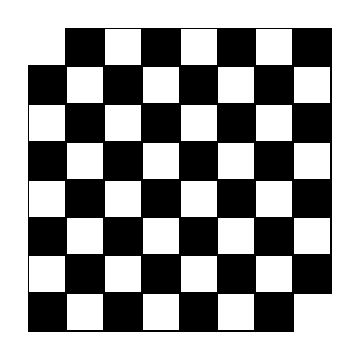
\begin{tikzpicture}[scale=0.48]
    \foreach \x in {0,...,7} {
        \foreach \y in {0,...,7} {
            \pgfmathsetmacro{\isCorner}{((\x==0 && \y==7) || (\x==7 && \y==0)) ? 1 : 0}
            \ifnum\isCorner=0
                \pgfmathsetmacro{\isBlack}{int(mod(\x+\y, 2) == 0 ? 1 : 0)}
                \ifnum\isBlack=1
                    \draw[fill=black, draw=black, line width=0.6pt] (\x, \y) rectangle ++(1, 1);
                \else
                    \draw[fill=white, draw=black, line width=0.6pt] (\x, \y) rectangle ++(1, 1);
                \fi
            \fi
        }
    }
\end{tikzpicture}
\end{center}

খেয়াল কর, কোনো দাবাবোর্ডের দুই বিপরীত কোণার দুইটি ঘর একই রঙের। ধরে নিই, আমাদের দাবাবোর্ডে দুই বিপরীত কোণার দুইটি সাদা রঙের ঘর নেই। তাহলে এই দাবাবোর্ডে মোট $30$টি সাদা এবং $32$টি কালো রঙের ঘর আছে। খেয়াল কর, যেকোনো $2 \times 1$ ডমিনো দাবাবোর্ডে যেভাবেই বসাও না কেন, ঠিক একটি সাদা ঘরকে এবং ঠিক একটি কালো ঘরকে ঢেকে রাখে। তার মানে আমাদের দাবাবোর্ডকে ডমিনো দিয়ে টাইল করা সম্ভব যদি এবং কেবল যদি দাবাবোর্ডে সমান সংখ্যক সাদা এবং কালো রঙের ঘর থেকে থাকে। কিন্তু আমাদের এই দাবাবোর্ড কি এই শর্ত পূরণ করে?\\

এখানে আমরা দাবাবোর্ডের সাদা-কালো রঙের বিন্যাস ব্যবহার করে সমস্যাটি সমাধান করেছি। আমাদের সমাধানে কিন্তু একটি ইনভ্যারিয়্যান্ট ব্যবহার করা হয়েছে। তোমরা কি বলতে পারবে কোথায়?\\

অলিম্পিয়াডে দাবাবোর্ড ছাড়াও বিভিন্ন আকারের গ্রিডে টাইলিং বিষয়ক সমস্যা দেখা যায়।

\begin{tcolorbox}[colframe=blue!80!blue]
টাইলিং বলতে একটি নির্দিষ্ট নিয়মে সম্পূর্ণ গ্রিড পলিমিনো দ্বারা ঢেকে ফেলাকে বোঝায়। এক্ষেত্রে প্রশ্নে অন্য কিছুর উল্লেখ না থাকলে কোনো দুইটি পলিমিনো একটি আরেকটির কোনো অংশ ঢেকে রাখতে পারবে না (ওভারল্যাপবিহীন) এবং কোনো পলিমিনোর কোনো অংশ গ্রিডের বাইরে থাকতে পারবে না।
\end{tcolorbox}

এ ধাঁচের সমস্যায় সম্পূর্ণ গ্রিডকে চাতুর্যপূর্ণভাবে কালারিং করে ঐ টাইলিং সম্পর্কে কিছু গুরুত্বপূর্ণ বৈশিষ্ট্য বের করে সমাধান করা হয়।\\

চল আরেকটি চমৎকার উদাহরণ দেখি।\\

\begin{tcolorbox}[colframe=black!80!green,title=উদাহরণ 1.2.2]
প্রমাণ কর যে, একটি $4 \times 11$ আয়তকে L-টেট্রামিনো দিয়ে টাইল করা সম্ভব নয়।
\end{tcolorbox}

$4 \times 11$ আয়তকে $4$টি সারি ও $11$টি কলামের একটি গ্রিড হিসেবে চিন্তা কর। আমরা প্রথম ও তৃতীয় সারির সবগুলো ঘরকে কালো এবং দ্বিতীয় ও চতুর্থ সারির সবগুলো ঘরকে সাদা রঙ করি। খেয়াল কর, যেকোনো L-টেট্রামিনোকে গ্রিডে বসালে সেটি হয় $3$টি কালো ও $1$টি সাদা ঘর অথবা $1$টি কালো ও $3$টি সাদা ঘরকে ঢেকে রাখবে। কিন্তু পুরো গ্রিডে সাদা ও কালো ঘরের সংখ্যা পরস্পর সমান। তার মানে, যদি কোনোভাবে সম্পূর্ণ গ্রিডকে টাইল করা সম্ভব হয় তাহলে দুই ধরনের তথা $3$টি কালো ও $1$টি সাদা ঘরবিশিষ্ট L-টেট্রামিনো এবং $1$টি কালো ও $3$টি সাদা ঘরবিশিষ্ট L-টেট্রামিনোর সংখ্যা সমান হতে হবে। অর্থাৎ, সর্বমোট L-টেট্রামিনোর সংখ্যা জোড় হতে হবে। কিন্তু $4 \times 11$ গ্রিডকে টাইল করা সম্ভব হলে ঠিক $11$টি L-টেট্রামিনো লাগতো, একটি কন্ট্রাডিকশন!\\

একটি বোর্ডকে একাধিক রকমের পলিমিনো দিয়েও টাইল করা যেতে পারে। পরবর্তী সমস্যায় এমনই একটি টাইলিং দেখতে পাবে।\\

\begin{tcolorbox}[colframe=black!80!green,title=উদাহরণ 1.2.3]
একটি $8 \times 8$ দাবাবোর্ডকে কি $15$টি $1 \times 4$ আয়ত এবং একটি $2 \times 2$ বর্গ দ্বারা টাইল করা যাবে?
\end{tcolorbox}

আশা করি এতক্ষণে সবাই অনুমান করতে পারছো যে এরকম টাইলিং করা সম্ভব নয়। অলিম্পিয়াডে একটি সমস্যায় একটি নির্দিষ্ট টাইলিং করা সম্ভব কিনা এটা জিজ্ঞেস করা হলে এর উত্তর সাধারণত না-ই হয়। এরকম সমস্যায় সাধারণত কালারিং টেকনিক ব্যবহার করে একটি কন্ট্রাডিকশনে উপনীত হতে হয়।\\

আমরা দাবাবোর্ডটিকে নিচের চিত্রের মতো করে রঙ করি।

\begin{center}
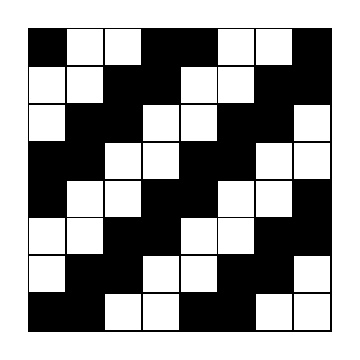
\begin{tikzpicture}[scale=0.48, line width=0.6pt]
    \foreach \x in {0,...,7} {
        \foreach \y in {0,...,7} {
            \pgfmathsetmacro{\val}{int(mod(mod(\x-\y, 4)+4, 4))}
            \ifnum\val<2
                \draw[fill=black, draw=black] (\x, \y) rectangle ++(1, 1);
            \else
                \draw[fill=white, draw=black] (\x, \y) rectangle ++(1, 1);
            \fi
        }
    }
\end{tikzpicture}
\end{center}

একটু খেয়াল করে দেখ, একটি $1 \times 4$ আয়তকে বোর্ডের যেকোনো স্থানে বসালে সেটা $2$টি করে সাদা এবং কালো ঘরকে ঢাকবে। আবার $2 \times 2$ বর্গকে বোর্ডের যেকোনো স্থানে বসালে সেটা হয় $1$টি সাদা ও $3$টি কালো অথবা $3$টি সাদা ও $1$টি কালো ঘরকে ঢাকবে। যদি এই টাইলিং করা সম্ভব হতো, তবে বোর্ডটিতে এই $16$টি টাইল মিলে হয় $31$টি সাদা ও $33$টি কালো অথবা $33$টি সাদা ও $31$টি কালো ঘরকে ঢেকে রাখতো। কিন্তু আমাদের কালারিংয়ে ঠিক $32$টি করে সাদা এবং কালো ঘর রয়েছে, একটি কন্ট্রাডিকশন!\\

এখন তোমাদের মনে প্রশ্ন জাগতে পারে, সঠিক কালারিং পেয়ে গেলে এ ধরনের সমস্যা সমাধান করা অনেক সহজ হয়ে যায়। কিন্তু কোন কালারিংটি প্রদত্ত সমস্যাটিতে কাজ করবে সেটা বুঝার উপায় কী?

\begin{tcolorbox}[colframe=blue!80!blue]
প্রচুর অনুশীলন করে নিজের সমস্যা সমাধানের দক্ষতা বাড়িয়ে নিলে তুমি কার্যকরী কালারিংটি সহজেই পেয়ে যাবে। নিজের ইন্টুইশন ব্যবহার করে বিভিন্ন ধরনের কালারিংয়ের জন্য চেক করে দেখ কোনো গুরুত্বপূর্ণ তথ্য বের হয়ে আসছে কিনা।
\end{tcolorbox}

\section{সিমেট্রি}

শুধুমাত্র একবার কালারিং করেই একটি সমস্যার সম্পূর্ণ সমাধান না-ও পেতে পার। সেক্ষেত্রে একাধিকবার কালারিং করা ছাড়াও আরও কিছু ট্রিক প্রয়োগ করতে হতে পারে।\\

\begin{tcolorbox}[colframe=black!80!green,title=Italy TST 1995]
একটি $8 \times 8$ দাবাবোর্ডকে $21$টি $3 \times 1$ ত্রিমিনো দিয়ে টাইল করা হয়েছে, যেন ঠিক একটি ঘর কোনো ত্রিমিনো দিয়ে ঢাকা না থাকে। কোনো দুইটি ত্রিমিনো একটি আরেকটির কোনো অংশ ঢেকে রাখতে পারবে না এবং কোনো ত্রিমিনোর কোনো অংশ বোর্ডের বাইরে থাকতে পারবে না। যে ঘরটি কোনো ত্রিমিনো দিয়ে ঢাকা নয় তার সম্ভাব্য সকল অবস্থান নির্ণয় কর।
\end{tcolorbox}

এক্ষেত্রে দাবাবোর্ডের সাদা-কালো রঙের বিন্যাস ব্যবহার করার চেষ্টা করলে তেমন লাভ হয় না। যেহেতু $3$ টালিবিশিষ্ট ত্রিমিনো দিয়ে টাইলিং করা হচ্ছে, সেহেতু $3$টি রঙ ব্যবহার করে দেখি কোনো লাভ হয় কিনা। চিত্রে এমন একটি কালারিং দেখানো হলো যেখানে $1, 2, 3$ দিয়ে $3$টি রঙ নির্দেশ করা হচ্ছে। (আমাদের সুবিধার্থে আমরা প্রত্যেকটি ঘরে রঙের বদলে সংখ্যা বসাতে পারি যেগুলো আসলে রঙের মতই কাজ করবে)

\begin{center}
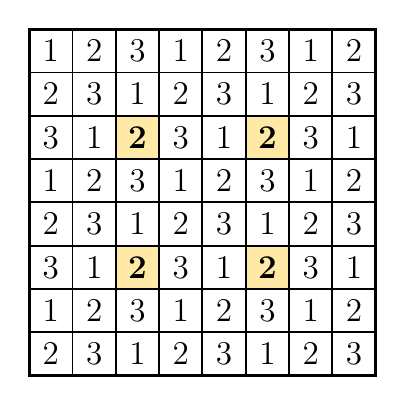
\begin{tikzpicture}[scale=0.55]
    \foreach \r in {0,...,7} {
        \foreach \c in {0,...,7} {
            \pgfmathsetmacro{\y}{7-\r}
            \pgfmathsetmacro{\num}{int(mod(\r+\c, 3) + 1)}
            \pgfmathsetmacro{\isSpecial}{((\r==2 && \c==2) || (\r==2 && \c==5) || (\r==5 && \c==2) || (\r==5 && \c==5)) ? 1 : 0}
            \ifnum\isSpecial=1
                \fill[amber!35] (\c, \y) rectangle ++(1, 1);
                \node at (\c+0.5, \y+0.5) {\large\textbf{\num}};
            \else
                \fill[white] (\c, \y) rectangle ++(1, 1);
                \node at (\c+0.5, \y+0.5) {\large \num};
            \fi
        }
    }
    \draw[draw=black, line width=0.7pt] (0, 0) grid (8, 8);
    \draw[draw=black, line width=1.1pt] (0, 0) rectangle (8, 8);
\end{tikzpicture}
\end{center}

খেয়াল করে দেখ, যেকোনো ত্রিমিনো প্রত্যেক রঙের ঠিক একটি করে ঘর ঢেকে রাখে। অর্থাৎ, টাইলিংয়ের পর প্রত্যেক রঙের ঠিক $21$টি করে ঘর ঢেকে রাখবে। কিন্তু চিত্রে $22$টি $2$, $21$টি $1$ এবং $21$টি $3$ আছে। তার মানে না-ঢাকা ঘরটাতে নিশ্চয় $2$ থাকতে হবে! আমাদের সমাধান কিন্তু শেষ হয়নি। আমরা কি $22$টি $2$ এর যেকোনোটিকে না ঢেকে রেখে সম্পূর্ণ দাবাবোর্ড টাইল করতে পারব?\\

না! সবগুলো $2$ এর অবস্থানের জন্য এটি সত্য নয়। কিন্তু সেটা প্রমাণ করব কীভাবে? ধর আমরা আমাদের শুরুর কালারিংটা নিয়ে বোর্ডের উল্লম্ব প্রতিসমতার অক্ষের সাপেক্ষে প্রতিফলন নিলাম। উদাহরণস্বরূপ সবচেয়ে উপরের সারিটি হয়ে যাবে $2, 1, 3, 2, 1, 3, 2, 1$ - অর্থাৎ পূর্বের কালারিংটিই উল্টোভাবে। আমাদের নতুন কালারিংয়েও একই যুক্তিতে না-ঢাকা ঘরটাতে $2$ থাকতে হবে। তার মানে উভয় কালারিংয়েই না-ঢাকা ঘরটাতে $2$ থাকতে হবে! খেয়াল কর এমন মাত্র $4$টি ঘরই রয়েছে, যেগুলো চিত্রে হাইলাইট করা আছে। এখন তোমাকে এই $4$টি ঘরের যেকোনো একটিকে না ঢেকে রেখে বাকি অংশ যে টাইল করা সম্ভব, সেটা দেখাতে হবে। এই কন্সট্রাকশনটুকু না হয় তোমরাই দেখানোর চেষ্টা কর।\\

আমরা এই সমস্যাতে ইনভ্যারিয়্যান্ট এর আইডিয়া ছাড়াও নতুন একটি টেকনিক ব্যবহার করেছি, যেটা হল সিমেট্রি বা প্রতিসমতা। পুরো চিত্রকে কখনো কখনো একটি প্রতিসমতার অক্ষের সাপেক্ষে উল্টিয়ে চিন্তা করলে সমাধানের জন্য গুরুত্বপূর্ণ কিছু তথ্য বের হতে পারে।

\section{ওভারল্যাপিং}

টাইলিংয়ের ক্ষেত্রে সবসময় যে একটি টাইলের কোনো অংশ অপর কোনো টাইলকে ঢাকতে পারবে না, তা কিন্তু সত্যি নয়। পরবর্তী উদাহরণে তোমরা কিছুটা ভিন্ন ধাঁচের টাইলিং দেখতে পারবে।\\

\begin{tcolorbox}[colframe=black!80!green,title=Russia 1996]
কোনো $5 \times 7$ বোর্ডকে কি L-ত্রিমিনো দিয়ে টাইল (ওভারল্যাপসহ) করা যাবে যেন কোনো L-ত্রিমিনোর কোনো অংশ বোর্ডের বাইরে না থাকে এবং বোর্ডের প্রতিটি ঘর সমসংখ্যক L-ত্রিমিনো দিয়ে ঢাকা থাকে?
\end{tcolorbox}

আমরা $5 \times 7$ বোর্ডকে নিচের চিত্রের মতো করে রঙ করি।

\begin{center}
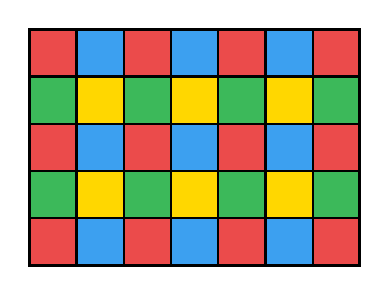
\begin{tikzpicture}[scale=0.6]
    \foreach \x in {0,...,6} {
        \foreach \y in {0,...,4} {
            \pgfmathsetmacro{\isYEven}{int(mod(\y, 2) == 0 ? 1 : 0)}
            \pgfmathsetmacro{\isXEven}{int(mod(\x, 2) == 0 ? 1 : 0)}
            \ifnum\isYEven=1
                \ifnum\isXEven=1
                    \fill[cellred] (\x, \y) rectangle ++(1, 1);
                \else
                    \fill[cellblue] (\x, \y) rectangle ++(1, 1);
                \fi
            \else
                \ifnum\isXEven=1
                    \fill[cellgreen] (\x, \y) rectangle ++(1, 1);
                \else
                    \fill[cellyellow] (\x, \y) rectangle ++(1, 1);
                \fi
            \fi
        }
    }
    \draw[draw=black, line width=0.8pt] (0, 0) grid (7, 5);
    \draw[draw=black, line width=1.1pt] (0, 0) rectangle (7, 5);
\end{tikzpicture}
\end{center}

দেখা যাচ্ছে যে বোর্ডের মোট $12$টি ঘরকে লাল রঙ করা হয়েছে। খেয়াল কর, একটি L-ত্রিমিনো বোর্ডে বসালে সেটা সর্বোচ্চ একটি লাল ঘরকে ঢাকতে পারবে (ওভারল্যাপ করা সব L-ত্রিমিনোই স্বাধীনভাবে ঐ ঘরকে ঢেকেছে ধরা হয়েছে)। যেহেতু বোর্ডের প্রতিটি ঘর সমান সংখ্যক L-ত্রিমিনো দিয়ে ঢাকা থাকবে, সুতরাং বোর্ডের উপর L-ত্রিমিনোর কয়েকটি স্তর সৃষ্টি হবে। ধরি, এরূপ $m$টি স্তরের সৃষ্টি হবে। যেহেতু L-ত্রিমিনোতে $3$টি টালি বিদ্যমান এবং $3 \nmid 5 \cdot 7 = 35$, তাই $m$ অবশ্যই $3$ দ্বারা বিভাজ্য হতে হবে। আমরা লিখতে পারি, $m = 3k$, যেখানে $k$ একটি ধনাত্মক পূর্ণসংখ্যা। তাহলে সর্বমোট L-ত্রিমিনোর সংখ্যা $\frac{3k \cdot 5 \cdot 7}{3} = 35k$টি। অর্থাৎ, সর্বোচ্চ $35k$ বার কোনো লাল ঘর ঢাকা সম্ভব। কিন্তু মোট $12 \cdot 3k = 36k$ বার লাল ঘর ঢাকতে হবে, একটি কন্ট্রাডিকশন!\\

এই সমস্যা সমাধানে আমরা ডবল কাউন্টিং টেকনিক ব্যবহার করেছি। তোমরা এ ব্যাপারে আরো জানতে চাইলে গুগল মামাকে জিজ্ঞেস কর।\\

\section{অসীম দাবাবোর্ড?}

অনেক সময় টাইলিং জাতীয় সমস্যায় কালারিংয়ের ক্ষেত্রে মোট রঙের সংখ্যা ও বিন্যাস একটি চলকের উপর নির্ভর করতে পারে।\\

\begin{tcolorbox}[colframe=black!80!green,title=Tournament of Towns 2009]
অরিত্র $2023$টি $n \times n$ কার্ডবোর্ডের টুকরা একটি অসীম দাবাবোর্ডে বসায় (ওভারল্যাপ হতে পারে), যেন প্রতিটি কার্ডবোর্ডের টুকরা ঠিক $n^2$ সংখ্যক ঘরকে ঢেকে রাখে। প্রমাণ কর যে, কমপক্ষে $n^2$ সংখ্যক ঘর রয়েছে যাদের প্রতিটিকে বেজোড়সংখ্যক কার্ডবোর্ডের টুকরা ঢেকে রেখেছে।
\end{tcolorbox}

এই সমস্যা সমাধানের ক্ষেত্রে $n$ এর জায়গায় কোনো ছোট একটি মান ধরে এবং $2023$ এর বেজোড় বৈশিষ্ট্য মাথায় রেখে $2023$ এর জায়গায় একটি ছোট বেজোড় সংখ্যা ব্যবহার করে সমাধান বের করার চেষ্টা করা উচিত। এই নতুন সমস্যাটির সমাধান করতে পারলে সমাধানটিকে সাধারণীকরণ করে যেকোনো $n$ এর জন্য সমাধানের আইডিয়া পাবে।\\

আমরা $(0, 0), (0, 1), \ldots, (n-1, n-1)$ লেবেলের এই $n^2$ টি রঙ ব্যবহার করব। অসীম দাবাবোর্ডকে আমরা স্থানাঙ্ক ব্যবস্থার সাথে তুলনা করতে পারি, যেখানে প্রতিটি ঘরকে একেকটি ল্যাটিস বিন্দু হিসেবে চিন্তা করা যায়। $(x, y)$ ঘরকে আমরা $(x \pmod n, y \pmod n)$ রঙ দিয়ে রঙ করি। খেয়াল কর, যেকোনো $n \times n$ গ্রিডে প্রতিটি রঙের ঠিক একটি করে ঘর রয়েছে। $2023$টি কার্ডবোর্ডের টুকরার মধ্যে যেকোনো টুকরাই প্রতিটি রঙের ঠিক একটি ঘরকে ঢেকে রাখে। তার মানে পিজিয়নহোল প্রিন্সিপল অনুযায়ী যেকোনো একটি রঙের এমন কিছু ঘর থাকতে হবে, যাদের প্রতিটিকে বেজোড়সংখ্যক কার্ডবোর্ডের টুকরা ঢেকে রেখেছে। অর্থাৎ, $n^2$ টি রঙের প্রতিটির অন্তত একটি করে ঘর আছে যাকে বেজোড়সংখ্যক কার্ডবোর্ডের টুকরা ঢেকে রেখেছে। সমাধান শেষ!\\

এখানে সমাধান লেখার সুবিধার্থে মডুলার অ্যারিথমেটিকের নোটেশন ব্যবহার করা হয়েছে।

\newpage

\section{অনুশীলনী}

\begin{flushleft}

\textbf{\textcolor{blue}{সমস্যা ১.}} প্রমাণ কর যে, একটি $10 \times 10$ বোর্ডকে $1 \times 4$ টেট্রামিনো দিয়ে টাইল করা সম্ভব নয়। T-টেট্রামিনো দিয়ে কি টাইল করা সম্ভব?

\textbf{\textcolor{blue}{সমস্যা ২.}} প্রমাণ কর যে, একটি $8 \times 8$ দাবাবোর্ডকে $15$টি T-টেট্রামিনো এবং একটি বর্গাকার টেট্রামিনো দ্বারা টাইল করা সম্ভব নয়।

\textbf{\textcolor{blue}{সমস্যা ৩.}} একটি $7 \times 7$ বোর্ড থেকে কোন ঘরটিকে সরালে বোর্ডের বাকি অংশটুকু $1 \times 3$ ত্রিমিনো দ্বারা টাইল করা যাবে?

\textbf{\textcolor{blue}{সমস্যা ৪.}} একটি $n \times n$ দাবাবোর্ডে চারকোণার চারটি ঘর নেই। এমন সকল $n$ বের কর যেন সম্পূর্ণ বোর্ডটি L-টেট্রামিনো দ্বারা টাইল করা সম্ভব।

\textbf{\textcolor{blue}{সমস্যা ৫.}} ফাহিম একটি $8 \times 9$ বোর্ডে ডমিনো বসাবে। কিন্তু সে খুব জেদী। নিচের চিত্রের মতো চিহ্নিত স্থানগুলোতে $6$টি ডমিনো তার বসাতেই হবে। ফাহিম বোর্ডে সর্বোচ্চ কয়টি ডমিনো বসাতে পারবে?

\begin{center}
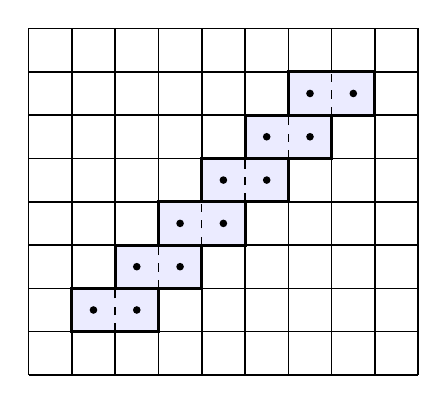
\begin{tikzpicture}[scale=0.55]
    \draw[draw=black, line width=0.6pt] (0,0) grid (9,8);
    \foreach \startX/\y in {1/1, 2/2, 3/3, 4/4, 5/5, 6/6} {
        \draw[fill=blue!8, draw=black, line width=1.1pt] (\startX, \y) rectangle ++(2, 1);
        \draw[draw=black, line width=0.5pt, dashed] (\startX+1, \y) -- (\startX+1, \y+1);
        \fill[black] (\startX+0.5, \y+0.5) circle (2.5pt);
        \fill[black] (\startX+1.5, \y+0.5) circle (2.5pt);
    }
\end{tikzpicture}
\end{center}

\textbf{\textcolor{blue}{সমস্যা ৬.}} একটি আয়তাকার মেঝে $2 \times 2$ এবং $1 \times 4$ টাইলস দ্বারা টাইল করা হয়েছে। অনুভব রাগের মাথায় একটি টাইল ভেঙ্গে ফেললো। তার কাছে অন্য টাইপের একটি টাইল আছে। সে কি এই নতুন টাইলটি সহ সবগুলো টাইলকে পুনর্বিন্যাস করে পুনরায় সম্পূর্ণ মেঝেকে টাইল করতে পারবে?

\textbf{\textcolor{blue}{সমস্যা ৭.}} একটি $66 \times 62$ আয়তকে কি $12 \times 1$ আয়ত দ্বারা টাইল করা যাবে?

\textbf{\textcolor{blue}{সমস্যা ৮.}} একটি $(2n-1) \times (2n-1)$ বোর্ডকে L-ত্রিমিনো, Z-টেট্রামিনো এবং বক্স টেট্রামিনো দ্বারা টাইল করা হল। প্রমাণ কর, কমপক্ষে $4n-1$ টি L-ত্রিমিনো লাগবে।

\textbf{\textcolor{blue}{সমস্যা ৯.}} একটি $(4k+2) \times (4k+2)$ বোর্ডকে কি T-টেট্রামিনো দিয়ে টাইল করা যাবে?

\textbf{\textcolor{blue}{সমস্যা ১০.}} একটি $23 \times 23$ বোর্ডকে $1 \times 1, 2 \times 2$ ও $3 \times 3$ টাইলস দ্বারা সম্পূর্ণভাবে টাইল করা হয়েছে। কমপক্ষে কয়টি $1 \times 1$ টাইল প্রয়োজন?

\textbf{\textcolor{blue}{সমস্যা ১১.}} দেখাও যে, একটি আয়ত যদি কিছুসংখ্যক ছোট আকারের আয়ত দিয়ে টাইল করা যায় যাদের প্রতিটির অন্তত একটি বাহুর দৈর্ঘ্য পূর্ণসংখ্যা, তাহলে টাইলকৃত আয়তের অন্তত একটি বাহুর দৈর্ঘ্য পূর্ণসংখ্যা।

\end{flushleft}

\chapter{কালারিংয়ের বিচিত্র কিছু প্রয়োগ}

\section{ঘুঁটি বসাও}

এমন অনেক সমস্যা আছে যেখানে কোনো বোর্ড বা গ্রিডে দাবার ঘুঁটি, পাথর বা অন্য কিছু বসানোর ব্যাপারে বলা হয়। কালারিং টেকনিক ব্যবহার করে এই ধরনের সমস্যা সমাধানে গুরুত্বপূর্ণ কিছু তথ্য বের করা যায়।\\

\begin{tcolorbox}[colframe=black!80!green,title=IMO 2018]
একটি \textit{সাইট} হলো সমতলের উপর এমন একটি বিন্দু $(x, y)$ যেন $0 < x, y \leq 20$। শুরুতে $400$টি সাইটের সবগুলোই খালি ছিল। গোমুজ এবং মুত্তাকিন পরপর খালি সাইটগুলোতে পাথর বসায় (গোমুজ শুরু করে)। গোমুজ পাথর বসানোর সময় যেকোনো একটি খালি সাইটে একটি লাল পাথর বসায় যেন দুইটি লাল পাথর বসানো সাইটের মধ্যবর্তী দূরত্ব $\sqrt{5}$ না হয়। মুত্তাকিন পাথর বসানোর সময় যেকোনো একটি খালি সাইটে নীল পাথর বসায় (দুইটি নীল পাথর বসানো সাইটের মধ্যবর্তী দূরত্ব $\sqrt{5}$ হতে পারে)। কোনো একজন পাথর বসাতে না পারলে তারা পাথর বসানো বন্ধ করে।\\

এমন সবচেয়ে বড় $K$ বের কর যেন মুত্তাকিন যেখানেই নীল পাথরগুলো বসাক না কেন, গোমুজ কমপক্ষে $K$টি লাল পাথর বসাতে পারবে।
\end{tcolorbox}

সমতলের উপর সাইটের সংজ্ঞার বদলে আমরা $20 \times 20$ একটি বোর্ড ব্যবহার করতে পারি, যেখানে সাইটগুলোকে এই বোর্ডের ঘর হিসেবে চিন্তা করতে পারি এবং দুইটি সাইটের মধ্যবর্তী দূরত্ব এর স্থলে দুইটি ঘরের মধ্যবিন্দুদ্বয়ের সংযোজক রেখার দৈর্ঘ্য ব্যবহার করতে পারি।\\

আমরা দেখাব যে, $K$ এর মান সর্বোচ্চ $100$ হতে পারে। চল প্রথমে আমরা দেখাই যে মুত্তাকিন যেখানেই নীল পাথরগুলো বসাক না কেন, গোমুজ কমপক্ষে $100$টি লাল পাথর বসাতে পারবে। এজন্য আমরা নিচের চিত্রের মতো দাবাবোর্ডের সাদা-কালো বিন্যাসে পুরো বোর্ডটিকে রঙ করি।\\

\begin{center}
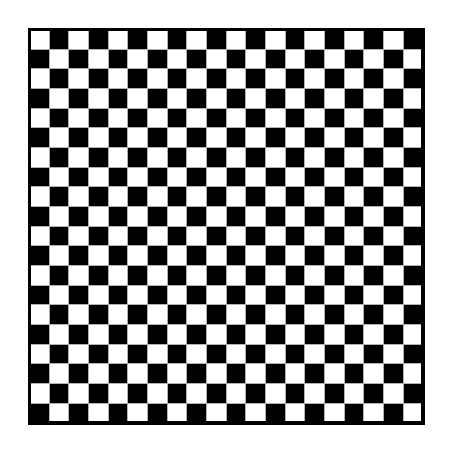
\begin{tikzpicture}[scale=0.25]
    \foreach \x in {0,...,19} {
        \foreach \y in {0,...,19} {
            \pgfmathsetmacro{\isBlack}{int(mod(\x+\y, 2) == 0 ? 1 : 0)}
            \ifnum\isBlack=1
                \fill[black] (\x, \y) rectangle ++(1, 1);
            \fi
        }
    }
    \draw[draw=black!30, line width=0.35pt] (0, 0) grid (20, 20);
    \draw[draw=black, line width=1.2pt] (0, 0) rectangle (20, 20);
\end{tikzpicture}
\end{center}

গোমুজ শুধুমাত্র সাদা ঘরগুলোতে লাল পাথর বসাবে। খেয়াল কর, কোনো দুইটি সাদা ঘরের মধ্যকার দূরত্ব $\sqrt{5}$ নয়। তার মানে গোমুজ লাল পাথর বসানোর জন্য কমপক্ষে $100$টি সাদা ঘর খালি পাবে।\\

এখন আমরা প্রমাণ করব যে, মুত্তাকিন নীল পাথরগুলো বসানোর জন্য এমনভাবে খালি ঘর নির্বাচন করতে পারবে যেন গোমুজ $100$টির বেশি লাল পাথর বসাতে পারবে না। তাই $20 \times 20$ বোর্ডটিকে $25$টি $4 \times 4$ বর্গে ভাগ করে ফেলি। এখন প্রতিটি বর্গকে নিচের চিত্রের মতো করে রঙ করি।\\

\begin{center}
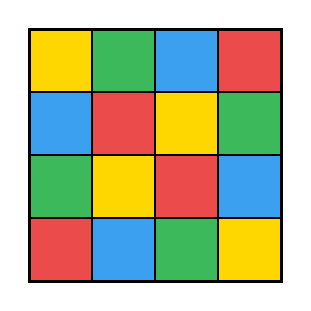
\begin{tikzpicture}[scale=0.8]
    \foreach \x/\y/\col in {
        0/3/cellyellow, 1/3/cellgreen, 2/3/cellblue, 3/3/cellred,
        0/2/cellblue, 1/2/cellred, 2/2/cellyellow, 3/2/cellgreen,
        0/1/cellgreen, 1/1/cellyellow, 2/1/cellred, 3/1/cellblue,
        0/0/cellred, 1/0/cellblue, 2/0/cellgreen, 3/0/cellyellow} {
        \fill[\col] (\x, \y) rectangle ++(1, 1);
    }
    \draw[draw=black, line width=0.8pt] (0, 0) grid (4, 4);
    \draw[draw=black, line width=1.1pt] (0, 0) rectangle (4, 4);
\end{tikzpicture}
\end{center}

খেয়াল কর একই রঙের যেকোনো চারটি ঘরের মধ্যবিন্দুগুলো যুক্ত করলে একটি রম্বস গঠিত হয় যার বাহুর দৈর্ঘ্য $\sqrt{5}$। গোমুজ যখনই একটি খালি ঘরে লাল পাথর বসাবে, মুত্তাকিন ঐ লাল পাথরবিশিষ্ট রম্বসের ঠিক বিপরীত খালি ঘরটিতে নীল পাথর বসাবে। অর্থাৎ গোমুজ একটি রম্বসের সর্বোচ্চ একটি খালি ঘরে লাল পাথর বসাতে পারবে। তাই গোমুজ সম্পূর্ণ বোর্ডে সর্বোচ্চ $\frac{1}{4} \cdot 400 = 100$টি ঘরে লাল পাথর বসাতে পারবে।\\

এই সমস্যা সমাধানে সবচেয়ে কঠিন অংশ ছিল দ্বিতীয় কালারিংটি বের করা। এই কালারিং বের করার পেছনে মোটিভেশন ছিল একটি দাবাবোর্ডে ঘোড়ার চাল নিয়ে চিন্তা করা। কারণ একটি ঘোড়ার চালের ক্ষেত্রে ঘোড়াটি সবসময় $\sqrt{5}$ একক দূরত্ব অতিক্রম করে।\\

\section{ঘোড়ার ভ্রমণ?}

একটি \textit{ঘোড়ার ভ্রমণ} বা \href{https://en.wikipedia.org/wiki/Knight%27s_tour}{Knight's Tour} বলতে দাবাবোর্ডের যেকোনো একটি ঘর থেকে একটি ঘোড়ার পরপর কিছুসংখ্যক চালকে বোঝায় যেন ঘোড়াটি দাবাবোর্ডের প্রতিটি ঘরকে ঠিক একবার পরিদর্শন করে। যদি ঘোড়াটি সম্পূর্ণ বোর্ড পরিদর্শন করে পরবর্তী চালেই শুরুর ঘরে ফিরে আসতে পারে তাহলে একে \textit{বদ্ধ} বা Closed, অন্যথায় একে \textit{খোলা} বা Open বলে। গুগল করে এরকম অনেক সিমুলেশন দেখে নিতে পারো। এখন চল \textit{ঘোড়ার ভ্রমণ} সম্পর্কিত একটি উদাহরণ দেখি।\\

\begin{tcolorbox}[colframe=black!80!green,title=উদাহরণ 2.2.1]
একটি $5 \times 5$ দাবাবোর্ডে কোনো \textit{বদ্ধ ঘোড়ার ভ্রমণ} আছে কি?
\end{tcolorbox}

না। শুধুমাত্র $5 \times 5$ দাবাবোর্ডে নয়, যেকোনো বেজোড়সংখ্যক ঘরবিশিষ্ট দাবাবোর্ডেই \textit{বদ্ধ ঘোড়ার ভ্রমণ} থাকা সম্ভব নয়! দাবাবোর্ডটিকে সাধারণ সাদা-কালো বিন্যাসে রঙ করি। খেয়াল কর, প্রতি চালে ঘোড়ার অবস্থান করা ঘরের রঙ বদলায়। তাই বেজোড়সংখ্যক চালের পর ঘোড়াটি শুরুর ঘরের বিপরীত রঙবিশিষ্ট ঘরে যেয়ে বসবে। ভ্রমণটি \textit{বদ্ধ ঘোড়ার ভ্রমণ} হতে হলে বেজোড়সংখ্যক চালের পর ঘোড়াটিকে শুরুর ঘরে পৌঁছাতে হবে, কিন্তু তা কখনো সম্ভব নয়। অর্থাৎ বেজোড়সংখ্যক ঘরবিশিষ্ট কোনো দাবাবোর্ডে \textit{বদ্ধ ঘোড়ার ভ্রমণ} থাকা সম্ভব নয়।\\

\section{থ্রিডি কালারিং?}

কিছু কিছু সমস্যায় বিভিন্ন আকৃতির ঘনবস্তু (যেমন-ইট) দিয়ে একটি বৃহদাকার বক্সকে প্যাক করা হয়। প্যাকিংকে ত্রিমাত্রিক টাইলিং হিসেবে চিন্তা করতে পারো। এক্ষেত্রে অন্য কিছু উল্লেখ করা না থাকলে বক্সটি সম্পূর্ণরূপে ভরাট করে প্যাক করতে হবে এবং প্যাকিংয়ের কাজে ব্যবহৃত ঘনবস্তুগুলোর কোনো অংশ বক্সটির আয়তনের বাইরে যেতে পারবে না। এধরনের সমস্যায়ও কালারিংয়ের ব্যবহার করা সম্ভব। নিচের উদাহরণটি দেখলেই বিষয়টা বুঝতে পারবে।\\

\begin{tcolorbox}[colframe=black!80!green,title=উদাহরণ 2.3.1]
একটি $6 \times 6 \times 6$ বক্সকে কি $54$টি $1 \times 1 \times 4$ আকৃতির ইট দ্বারা প্যাক করা যাবে?
\end{tcolorbox}

আমরা বক্সটিকে একটি ঘনক হিসেবে চিন্তা করতে পারি। একটি $6 \times 6 \times 6$ ঘনকে $27$টি $2 \times 2 \times 2$ উপঘনক বিদ্যমান। উপঘনকগুলোকে আমরা দাবাবোর্ডের মত পরপর সাদা-কালো রঙে রঙ করতে পারি। ধরি, এক্ষেত্রে $14$টি উপঘনক কালো রঙ এবং $13$টি উপঘনক সাদা রঙ করা হবে। অর্থাৎ, মোট $112$টি কালো এবং $104$টি সাদা একক ঘনক থাকবে। খেয়াল কর, একটি $1 \times 1 \times 4$ আকৃতির ইট বক্সের যেকোনো স্থানে বসালে সেটি ঠিক $2$টি কালো এবং $2$টি সাদা একক ঘনকের জায়গা দখল করবে। তার মানে, $54$টি ইট দ্বারা প্যাকিং করা সম্ভব হলে সেগুলো মোট $108$টি সাদা একক ঘনকের জায়গা দখল করত। কিন্তু বক্সে $104$টি সাদা একক ঘনক আছে, একটি কন্ট্রাডিকশন!\\

\section{ওজনের ব্যবহার}

\textit{ওজন} বা \href{https://en.wikipedia.org/wiki/Weight_function#:~:text=A%20weight%20function%20is%20a,weighted%20sum%20or%20weighted%20average.}{Weight} কালারিংয়েরই একটি ভিন্ন রূপ। এখানে ওজন কোনো আক্ষরিক অর্থ প্রকাশ করছে না, এটি একটি কনভেনশন। এক্ষেত্রে আমরা বিভিন্ন রঙ ব্যবহার করার বদলে \href{https://en.wikipedia.org/wiki/Root_of_unity}{এককের জটিল মূল} ব্যবহার করি। এই দুই পদ্ধতির সমাধান প্রকৃতপক্ষে একই। নিচের উদাহরণটি দেখলেই বিষয়টি বুঝতে পারবে।\\

\begin{tcolorbox}[colframe=black!80!green,title=উদাহরণ 2.4.1]
প্রমাণ কর যে, একটি $m \times n$ বোর্ডকে $1 \times k$ ডমিনো দিয়ে টাইল করা যাবে, যদি ও কেবল যদি $k \mid m$ অথবা $k \mid n$ হয়।
\end{tcolorbox}

আমরা এই সমস্যাটি দুইভাবে সমাধান করব। প্রথম পদ্ধতিতে আগের মতই $1, 2, 3, \ldots, k$ এই $k$টি রঙ ব্যবহার করব। নিচে $k=3$ এর জন্য কালারিং দেখানো হল।

\begin{center}
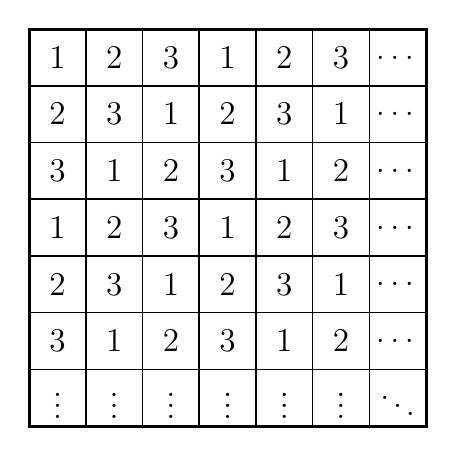
\begin{tikzpicture}[scale=0.72]
    \foreach \r in {0,...,5} {
        \foreach \c in {0,...,5} {
            \pgfmathsetmacro{\y}{6-\r}
            \pgfmathsetmacro{\num}{int(mod(\r+\c, 3) + 1)}
            \node at (\c+0.5, \y+0.5) {\large \num};
        }
        \node at (6.5, 6-\r+0.5) {\large $\dots$};
    }
    \foreach \c in {0,...,5} {
        \node at (\c+0.5, 0.5) {\large $\vdots$};
    }
    \node at (6.5, 0.5) {\large $\ddots$};
    \draw[draw=black, line width=0.6pt] (0, 0) grid (7, 7);
    \draw[draw=black, line width=1.1pt] (0, 0) rectangle (7, 7);
\end{tikzpicture}
\end{center}

খেয়াল কর, যেকোনো টাইল প্রতিটি রঙের ঠিক একটি করে ঘর ঢেকে রাখে। তার মানে, সম্পূর্ণ বোর্ডে প্রতিটি রঙের সমান সংখ্যক ঘর থাকতে হবে। এই শর্ত পূরণ হবে যদি এবং কেবল যদি $m$ অথবা $n$, $k$ দ্বারা বিভাজ্য হয় (এটা নিজেরা দেখানোর চেষ্টা কর)।\\

আমরা এখানে কালারিং পদ্ধতি ব্যবহার করার বদলে ওজন ব্যবহার করতে পারি। ধরি, এককের $k$ তম একটি মূল $\omega$। আগের পদ্ধতির $k$টি রঙের বদলে আমরা $1, \omega, \omega^2, \ldots, \omega^{k-1}$ এই $k$টি ওজন পরপর বসাই। নিচে $k=3$ এর জন্য ওজন বসানোর পদ্ধতি দেখানো হল।

\begin{center}
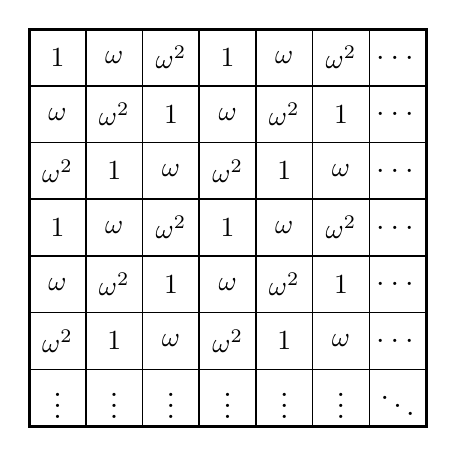
\begin{tikzpicture}[scale=0.72]
    \foreach \r in {0,...,5} {
        \foreach \c in {0,...,5} {
            \pgfmathsetmacro{\y}{6-\r}
            \pgfmathsetmacro{\num}{int(mod(\r+\c, 3) + 1)}
            \ifnum\num=1
                \node at (\c+0.5, \y+0.5) {$1$};
            \fi
            \ifnum\num=2
                \node at (\c+0.5, \y+0.5) {$\omega$};
            \fi
            \ifnum\num=3
                \node at (\c+0.5, \y+0.5) {$\omega^2$};
            \fi
        }
        \node at (6.5, 6-\r+0.5) {\large $\dots$};
    }
    \foreach \c in {0,...,5} {
        \node at (\c+0.5, 0.5) {\large $\vdots$};
    }
    \node at (6.5, 0.5) {\large $\ddots$};
    \draw[draw=black, line width=0.6pt] (0, 0) grid (7, 7);
    \draw[draw=black, line width=1.1pt] (0, 0) rectangle (7, 7);
\end{tikzpicture}
\end{center}

খেয়াল কর, যেকোনো টাইল প্রতিটি ওজনের ঠিক একটি করে ঘর ঢেকে রাখে। কিন্তু এভাবে ওজন বসিয়ে আমাদের লাভ কী হলো? আমরা তো রঙ বসিয়ে একই ধরনের ফল পেয়েছি। ওজন বসানোর ফায়দা একটি সূত্রে নিহিত।\\

\begin{tcolorbox}[colframe=blue!80!blue]
এককের যেকোনো $k$ তম মূল $\omega$ এর জন্য $$1+ \omega +\omega^2+ \ldots+\omega^{k-1} = 0$$
\end{tcolorbox}

অর্থাৎ প্রতিটি টাইল মোট $0$ ওজনের ঘর ঢেকে রাখবে। তার মানে সম্পূর্ণ বোর্ডের সব ওজনের সমষ্টি $0$! এখান থেকে আগের মতই কাঙ্ক্ষিত ফলাফল দেখানো সম্ভব (বীজগাণিতিক ক্যালকুলেশনটুকু নিজেরা করার চেষ্টা কর)।\\

কালারিং এবং ওজন ব্যবহার অনুরূপ হলেও কিছু কিছু সমস্যায় বীজগাণিতিক হিসাব করার সুযোগ থাকায় ওজন ব্যবহার করা সুবিধাজনক।

\newpage

\section{অনুশীলনী}

\begin{flushleft}

\textbf{\textcolor{blue}{সমস্যা ১.}} কোন স্বাভাবিক সংখ্যা $n$ এর জন্য একটি $4 \times n$ দাবাবোর্ডে একটি \textit{বদ্ধ ঘোড়ার ভ্রমণ} আছে?

\textbf{\textcolor{blue}{সমস্যা ২.}} একটি $10 \times 10 \times 10$ বক্সকে কি $250$টি $1 \times 1 \times 4$ আকৃতির ইট দ্বারা প্যাক করা যাবে?

\textbf{\textcolor{blue}{সমস্যা ৩.}} একটি $a \times b$ বোর্ডকে কিছু $n \times 1$ এবং $1 \times m$ ডমিনো দ্বারা টাইল করা যায় (ডমিনো ঘুরানো যাবে না)। প্রমাণ কর, $n \mid a$ অথবা $m \mid b$.

\textbf{\textcolor{blue}{সমস্যা ৪.}} একটি $9 \times 9$ দাবাবোর্ডের প্রতিটি ঘরে একটি করে পিঁপড়া রয়েছে। ওয়াহিদুল বোর্ডের নিচে টোকা দিলে প্রতিটি পিঁপড়া যেকোনো একদিকে কোণাকোণি পাশের ঘরে যায়। তখন এমন হতে পারে যে, কিছু ঘরে একাধিক পিঁপড়া আছে আবার কিছু ঘরে কোনো পিঁপড়া নেই। সম্ভাব্য সর্বনিম্ন পিঁপড়াবিহীন ঘরের সংখ্যা নির্ণয় কর।

\textbf{\textcolor{blue}{সমস্যা ৫.}} একটি $6 \times 6$ বোর্ড ডমিনো দ্বারা টাইল করা হয়েছে। দেখাও যে, এমন একটি সরলরেখা আছে যে বরাবর ছুরি চালালে কোনো ডমিনো না কেটে বোর্ডটিকে দুই ভাগে ভাগ করা যাবে। (ধরে নাও বোর্ড এবং ডমিনোগুলো রাবারের তৈরি) এই সরলরেখাকে \textit{ফল্ট লাইন} বলা হয়।

\textbf{\textcolor{blue}{সমস্যা ৬.} \textcolor{magenta}{(BdMO 2019 P10)}} দাবায় একটি সাধারণ ঘোড়া দুই ঘর সামনে এগিয়ে এক ঘর পাশে যায় যেকোন একদিকে। হাসিনের মনে হলো যে খেলাটাকে একটু জম্পেশ বানানো দরকার, তাই সে \textit{যোদ্ধা} নামে একটি নতুন ঘুঁটি বানালো। যোদ্ধা হয় তিন ঘর এগিয়ে এক ঘর পাশে যায় অথবা দুই ঘর এগিয়ে দুই ঘর পাশে যায় যেকোনো দিকে।

প্রমাণ কর যে, একটি $2020 \times 2020$ দাবাবোর্ডে সর্বোচ্চ যে সংখ্যক যোদ্ধা রাখা যায় যাতে তারা একে অপরকে আক্রমণ না করে তা ঘরের সংখ্যার $2/5$ অংশের সমান বা কম।

\textbf{\textcolor{blue}{সমস্যা ৭.} \textcolor{magenta}{(IMO SL 2010)}} $2500$টি রাজার ঘুঁটি একটি $100 \times 100$ দাবাবোর্ডে এমনভাবে সাজানো হয়েছে যেন

i. কোনো রাজা অন্য কোনো রাজাকে খেতে পারবে না (অর্থাৎ কোনো রাজার চারপাশের কোনো ঘরে অন্য কোনো রাজা নেই)।

ii. প্রতিটি সারি ও প্রতিটি কলামে $25$টি করে রাজা রয়েছে।

এমন কতভাবে বোর্ডটি সাজানো সম্ভব?

\textbf{\textcolor{blue}{সমস্যা ৮.} \textcolor{magenta}{(IMO 1993)}}
অর্ণব একটি অসীম দাবাবোর্ডে Solitaire খেলছে। খেলার শুরুতে $n^2$টি ঘুঁটি বোর্ডের উপর একটি $n$ একক বাহুবিশিষ্ট বর্গের প্রতিটি ঘর দখল করে আছে। অর্ণব প্রতি চালে যেকোনো একটি ঘুঁটি নিয়ে একটি দখলকৃত ঘর ডিঙিয়ে একটি খালি ঘর দখল করতে পারে এবং সে যে ঘুঁটি ডিঙিয়ে চাল দিয়েছে সেই ঘুঁটিটি বোর্ড থেকে সরিয়ে ফেলে। $n$ এর কোন মানের জন্য সম্পূর্ণ বোর্ডে একটি ঘুঁটি অবশিষ্ট থেকে খেলা শেষ হওয়া সম্ভব?

\textbf{\textcolor{blue}{সমস্যা ৯.} \textcolor{magenta}{(The Art Gallery Problem)}} একটি আর্ট গ্যালারি সরল n-ভুজ আকৃতির। গ্যালারির আকৃতি যত জটিলই হোক না কেন, এটিকে পাহারা দিতে কতজন প্রহরী থাকাই যথেষ্ট?

\end{flushleft}

\chapter{অলিম্পিয়াডের কিছু সমস্যা}

আমরা এই অধ্যায় কঠিন কিছু অলিম্পিয়াড প্রবলেম কিভাবে সমাধান করতে হয় তা দেখব।

\section{IMO এর ছড়াছড়ি}

এখন আমরা একটি কিউট আইএমও প্রবলেম দেখব। এটি ২০১৬ সালের আইএমও এর ২ নম্বর সমস্যা ছিল।\\

\begin{tcolorbox}[colframe=black!80!green,title=IMO 2016]
এমন সকল ধনাত্মক পূর্ণসংখ্যা $n$ বের কর যেন একটি $n \times n$ বোর্ডের প্রতিটি ঘরে $I, M$ ও $O$- এই তিনটি বর্ণের যেকোনো একটি বসানো যায়, যাতে নিচের শর্তগুলো পূরণ করে-\\

i. প্রতিটি সারি এবং প্রতিটি কলামে এক-তৃতীয়াংশ ঘরে $I$, এক-তৃতীয়াংশ ঘরে $M$ এবং এক-তৃতীয়াংশ ঘরে $O$ থাকবে।

ii. কোনো কর্ণের মোট ঘরের সংখ্যা তিনের গুণিতক হলে, এক-তৃতীয়াংশ ঘরে $I$, এক-তৃতীয়াংশ ঘরে $M$ এবং এক-তৃতীয়াংশ ঘরে $O$ থাকবে।
\end{tcolorbox}

এই সমস্যাটি নিয়ে কিছুক্ষণ কাজ করলে বুঝতে পারবে যে, শর্ত পূরণ করতে হলে $n$, $9$ দ্বারা বিভাজ্য হতে হবে। আমরা \textit{ওজন} ব্যবহার করে এটি প্রমাণ করব।\\

ধরি, $\omega = e^{\frac{2\pi i}{3}}$ এককের একটি ঘনমূল। এখন এমন একটি বোর্ড চিন্তা কর যাতে সকল শর্ত পূরণ করে ঘর ভরাট করা সম্ভব। আমরা $I$ এর জায়গায় $1$, $M$ এর জায়গায় $\omega$ এবং $O$ এর জায়গায় $\omega^2$ বসাই। তিনটি বাস্তব সংখ্যা $a, b, c$ এর জন্য $a+b\omega+c\omega^2 = 0$ যদি এবং কেবল যদি $a=b=c$ (বিশ্বাস না হলে প্রমাণ করার চেষ্টা কর!)। সুতরাং, প্রতিটি সারি, প্রতিটি কলাম এবং প্রতি তৃতীয় কর্ণের ওজনগুলোর যোগফল $0$। আবার খেয়াল কর, প্রতি সারিতে তিনের গুণিতক সংখ্যক ঘর রয়েছে, অর্থাৎ $3 \mid n$।\\

আমাদের হাতে অনেকগুলো সমীকরণ আছে। এতগুলো সমীকরণ নিয়ে একসাথে কাজ করা অনেক কঠিন হয়ে দাঁড়ায়। তাই আমরা সবচেয়ে সরলভাবে চিন্তা করার চেষ্টা করি। একটা আইডিয়া হতে পারে পুরো বোর্ডের সবগুলো সংখ্যা যোগ করে যোগফল $0$ হতে হবে সেটা বের করা। কিন্তু এভাবে খুব একটা কাজের জিনিস বের হয় না, কারণ এই বিষয়টা সত্য হতে হলে আমাদের সবগুলো শর্ত সত্য হওয়ার প্রয়োজন নেই। তাই আমরা আরেকটি আইডিয়া ব্যবহার করার চেষ্টা করি, যেখানে আমরা প্রতি তৃতীয় সমীকরণকে একত্রে গ্রুপ করব। ধরি, $a_{ij}$ হলো সকল $(i', j')$ ঘরের ভরগুলোর যোগফল যেখানে $i' \equiv i \pmod$ এবং $j' \equiv j \pmod$ যেখানে $1 \leq i, j \leq 3$। আমাদের সমীকরণগুলোকে সাজিয়ে নিচের মত করে লিখতে পারি।\\

$$ a_{11} + a_{12} + a_{13} = 0 \hspace{5cm}(1)$$
$$ a_{21} + a_{22} + a_{23} = 0 \hspace{5cm}(2)$$
$$ a_{31} + a_{32} + a_{33} = 0 \hspace{5cm}(3)$$
$$ a_{11} + a_{21} + a_{31} = 0 \hspace{5cm}(4)$$
$$ a_{12} + a_{22} + a_{32} = 0 \hspace{5cm}(5)$$
$$ a_{13} + a_{23} + a_{33} = 0 \hspace{5cm}(6)$$
$$ a_{11} + a_{22} + a_{33} = 0 \hspace{5cm}(7)$$
$$ a_{31} + a_{22} + a_{13} = 0 \hspace{5cm}(8)$$

এখন আমরা কোনো একটি চলকের মান বের করতে পারি কিনা চেষ্টা করি।

$$0 = (1) + (3) + (4) + (6) - 2 \cdot (7) - 2 \cdot (8) - (2) - (5) = -6a_{22}$$

অর্থাৎ, $a_{22} = 0$ কিন্তু তার মানে যে ঘরগুলোর ইনডেক্সদ্বয়  $3$ দ্বারা ভাগ করলে ভাগশেষ $2$ হয়, সেগুলোতে সমান সংখ্যক $I, M$ ও $O$ থাকতে হবে। সুতরাং, $\frac{n^2}{9}$, $3$ দ্বারা বিভাজ্য হতে হবে, তার মানে $9 \mid n$।\\

সমাধান কি শেষ হয়ে গেছে? না, হয়নি। আমরা প্রমাণ করেছি যে, শর্ত পূরণ করতে হলে $n$ অবশ্যই $9$ দ্বারা বিভাজ্য হতে হবে। কিন্তু শুধুমাত্র $n$, $9$ দ্বারা বিভাজ্য হলেই যে সকল শর্ত পূরণ করে প্রতিটি ঘরে বর্ণ বসানো যাবে, তা কিন্তু এখনো প্রমাণ হয়নি। সেটা প্রমাণ করার জন্য নিচের চিত্রের মতো $\frac{n^2}{81}$টি কপি সাজিয়ে সম্পূর্ণ বোর্ড শর্তানুযায়ী পূরণ করা যাবে।

\begin{center}
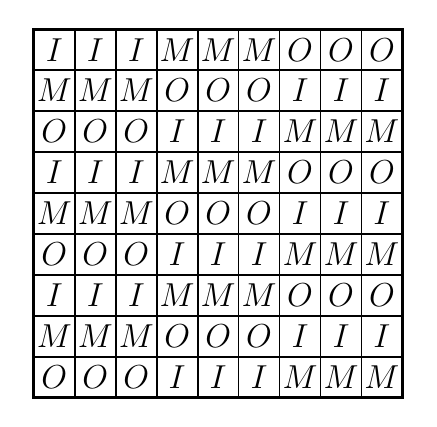
\begin{tikzpicture}[scale=0.52]
    \foreach \r in {0,...,8} {
        \foreach \c in {0,...,8} {
            \pgfmathsetmacro{\y}{8-\r}
            \pgfmathsetmacro{\bc}{int(\c/3)}
            \pgfmathsetmacro{\val}{int(mod(\r+\bc, 3))}
            \ifnum\val=0
                \node at (\c+0.5, \y+0.5) {\large $I$};
            \fi
            \ifnum\val=1
                \node at (\c+0.5, \y+0.5) {\large $M$};
            \fi
            \ifnum\val=2
                \node at (\c+0.5, \y+0.5) {\large $O$};
            \fi
        }
    }
    \draw[draw=black, line width=0.6pt] (0,0) grid (9,9);
    \draw[line width=1.1pt, draw=black] (0,0) rectangle (9,9);
\end{tikzpicture}
\end{center}

কোন ঘরগুলোতে সমান সংখ্যক $I, M$ ও $O$ আছে দেখানো লাগবে, সেটা বুঝতে পারার পর ওজন ব্যবহার করার বদলে ডবল কাউন্টিং টেকনিক ব্যবহার করেও সমাধান করা যায়।

\section{খোঁড়া নৌকা?}

এখন আমরা একটি আইএমও শর্টলিস্টেড প্রবলেম দেখে এই অধ্যায়টি শেষ করব। এটি ২০০৯ সালের আইএমও শর্টলিস্টের কম্বিনেটরিক্স অংশের ৬ নম্বর সমস্যা ছিল।\\

\begin{tcolorbox}[colframe=black!80!green,title=IMO SL 2009]
একটি $999 \times 999$ দাবাবোর্ডে একটি \textit{খোঁড়া নৌকা} নিচের মত করে চলতে পারে:

যেকোনো ঘর থেকে এটি এর পাশের যেকোনো একটি ঘরে যেতে পারে (পাশের ঘর বলতে সাধারণ বাহু বিশিষ্ট ঘরকে বোঝানো হয়েছে) এবং প্রতিটি চালই যেন একটি \textit{মোড়} হয় (অর্থাৎ পরপর দুইটি চালের দিক পরস্পর লম্ব হতে হবে)। একটি \textit{নিশ্ছেদ রুট} দিয়ে একটি নির্দিষ্ট ক্রমে পরপর পরস্পর ভিন্ন কিছুসংখ্যক ঘরকে বোঝায় যেগুলো একটি খোঁড়া নৌকা ঐ ক্রমে পরিদর্শন করতে পারবে। এমন একটি নিশ্ছেদ রুটকে \textit{চাক্রিক} বলা হয় যদি একটি খোঁড়া নৌকা রুটের শেষ ঘরটিতে পৌঁছানোর পর সরাসরি রুটের শুরুর ঘরটিতে যেতে পারবে এবং পুনরায় একই পথে চলা শুরু করতে পারবে। একটি খোঁড়া নৌকা সবচেয়ে দীর্ঘ চাক্রিক, নিশ্ছেদ রুটে মোট কয়টি ঘর পরিদর্শন করে?
\end{tcolorbox}

এখানে আমরা এরিক শেনের (AoPS User: \href{https://artofproblemsolving.com/community/user/265663}{TheUltimate123}) সমাধানটি দেখব।\\

একটি খোঁড়া নৌকা $999 \times 999$ দাবাবোর্ডে সবচেয়ে দীর্ঘ চাক্রিক, নিশ্ছেদ রুটে মোট $996000$টি ঘর পরিদর্শন করবে। আমরা এখানে এই সমস্যাটির আরো সাধারণীকৃত একটি ভার্সন সমাধান করব। আমরা দেখাব যে, $n \equiv 3 \pmod 4$ এবং $n \geq 7$ এর জন্য একটি $n \times n$ বোর্ডে এর উত্তর $n^2 - 2n -3.$\\

আমরা প্রথমে দেখাব যে, এমন একটি $n^2-2n-3$ টি ঘরবিশিষ্ট চাক্রিক, নিশ্ছেদ রুট আসলেই আছে। $n = 15$ এর জন্য আমাদের কন্সট্রাকশনটি নিম্নরূপ।

\begin{center}
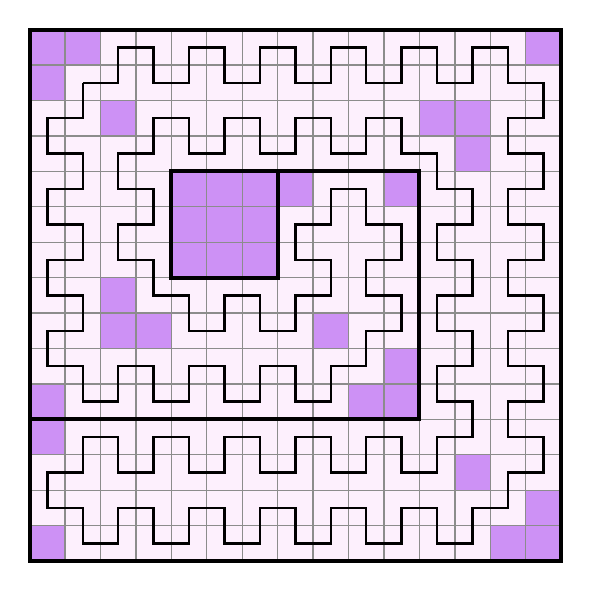
\begin{tikzpicture}[scale=0.45]
    \fill[snakelightpink] (0, 0) rectangle (15, 15);

    \fill[snakepurple] (4, 8) rectangle (7, 11);

    \foreach \x/\y in {
        0/0, 0/3, 0/4, 0/13, 0/14, 1/14, 2/6, 2/7, 2/12, 3/6,
        7/10, 8/6, 9/4, 10/4, 10/5, 10/10, 11/12, 12/2, 12/11, 12/12,
        13/0, 14/0, 14/1, 14/14
    } {
        \fill[snakepurple] (\x, \y) rectangle ++(1, 1);
    }

    \draw[draw=black!45, line width=0.5pt] (0, 0) grid (15, 15);

    \draw[line width=1.4pt, draw=black] (0, 0) rectangle (15, 15);
    \draw[line width=1.4pt, draw=black] (0, 4) -- (11, 4) -- (11, 11) -- (4, 11);
    \draw[line width=1.4pt, draw=black] (4, 8) rectangle (7, 11);

    \draw[line width=0.9pt, draw=black]
        (1.5, 13.5) -- (2.5, 13.5) -- (2.5, 14.5) -- (3.5, 14.5) -- (3.5, 13.5)
        -- (4.5, 13.5) -- (4.5, 14.5) -- (5.5, 14.5) -- (5.5, 13.5)
        -- (6.5, 13.5) -- (6.5, 14.5) -- (7.5, 14.5) -- (7.5, 13.5)
        -- (8.5, 13.5) -- (8.5, 14.5) -- (9.5, 14.5) -- (9.5, 13.5)
        -- (10.5, 13.5) -- (10.5, 14.5) -- (11.5, 14.5) -- (11.5, 13.5)
        -- (12.5, 13.5) -- (12.5, 14.5) -- (13.5, 14.5) -- (13.5, 13.5)
        -- (14.5, 13.5) -- (14.5, 12.5) -- (13.5, 12.5) -- (13.5, 11.5)
        -- (14.5, 11.5) -- (14.5, 10.5) -- (13.5, 10.5) -- (13.5, 9.5)
        -- (14.5, 9.5) -- (14.5, 8.5) -- (13.5, 8.5) -- (13.5, 7.5)
        -- (14.5, 7.5) -- (14.5, 6.5) -- (13.5, 6.5) -- (13.5, 5.5)
        -- (14.5, 5.5) -- (14.5, 4.5) -- (13.5, 4.5) -- (13.5, 3.5)
        -- (14.5, 3.5) -- (14.5, 2.5) -- (13.5, 2.5) -- (13.5, 1.5)
        -- (12.5, 1.5) -- (12.5, 0.5) -- (11.5, 0.5) -- (11.5, 1.5)
        -- (10.5, 1.5) -- (10.5, 0.5) -- (9.5, 0.5) -- (9.5, 1.5)
        -- (8.5, 1.5) -- (8.5, 0.5) -- (7.5, 0.5) -- (7.5, 1.5)
        -- (6.5, 1.5) -- (6.5, 0.5) -- (5.5, 0.5) -- (5.5, 1.5)
        -- (4.5, 1.5) -- (4.5, 0.5) -- (3.5, 0.5) -- (3.5, 1.5)
        -- (2.5, 1.5) -- (2.5, 0.5) -- (1.5, 0.5) -- (1.5, 1.5)
        -- (0.5, 1.5) -- (0.5, 2.5) -- (1.5, 2.5) -- (1.5, 3.5)
        -- (2.5, 3.5) -- (2.5, 2.5) -- (3.5, 2.5) -- (3.5, 3.5)
        -- (4.5, 3.5) -- (4.5, 2.5) -- (5.5, 2.5) -- (5.5, 3.5)
        -- (6.5, 3.5) -- (6.5, 2.5) -- (7.5, 2.5) -- (7.5, 3.5)
        -- (8.5, 3.5) -- (8.5, 2.5) -- (9.5, 2.5) -- (9.5, 3.5)
        -- (10.5, 3.5) -- (10.5, 2.5) -- (11.5, 2.5) -- (11.5, 3.5)
        -- (12.5, 3.5) -- (12.5, 4.5) -- (11.5, 4.5) -- (11.5, 5.5)
        -- (12.5, 5.5) -- (12.5, 6.5) -- (11.5, 6.5) -- (11.5, 7.5)
        -- (12.5, 7.5) -- (12.5, 8.5) -- (11.5, 8.5) -- (11.5, 9.5)
        -- (12.5, 9.5) -- (12.5, 10.5) -- (11.5, 10.5) -- (11.5, 11.5)
        -- (10.5, 11.5) -- (10.5, 12.5) -- (9.5, 12.5) -- (9.5, 11.5)
        -- (8.5, 11.5) -- (8.5, 12.5) -- (7.5, 12.5) -- (7.5, 11.5)
        -- (6.5, 11.5) -- (6.5, 12.5) -- (5.5, 12.5) -- (5.5, 11.5)
        -- (4.5, 11.5) -- (4.5, 12.5) -- (3.5, 12.5) -- (3.5, 11.5)
        -- (2.5, 11.5) -- (2.5, 10.5) -- (3.5, 10.5) -- (3.5, 9.5)
        -- (2.5, 9.5) -- (2.5, 8.5) -- (3.5, 8.5) -- (3.5, 7.5)
        -- (4.5, 7.5) -- (4.5, 6.5) -- (5.5, 6.5) -- (5.5, 7.5)
        -- (6.5, 7.5) -- (6.5, 6.5) -- (7.5, 6.5) -- (7.5, 7.5)
        -- (8.5, 7.5) -- (8.5, 8.5) -- (7.5, 8.5) -- (7.5, 9.5)
        -- (8.5, 9.5) -- (8.5, 10.5) -- (9.5, 10.5) -- (9.5, 9.5)
        -- (10.5, 9.5) -- (10.5, 8.5) -- (9.5, 8.5) -- (9.5, 7.5)
        -- (10.5, 7.5) -- (10.5, 6.5) -- (9.5, 6.5) -- (9.5, 5.5)
        -- (8.5, 5.5) -- (8.5, 4.5) -- (7.5, 4.5) -- (7.5, 5.5)
        -- (6.5, 5.5) -- (6.5, 4.5) -- (5.5, 4.5) -- (5.5, 5.5)
        -- (4.5, 5.5) -- (4.5, 4.5) -- (3.5, 4.5) -- (3.5, 5.5)
        -- (2.5, 5.5) -- (2.5, 4.5) -- (1.5, 4.5) -- (1.5, 5.5)
        -- (0.5, 5.5) -- (0.5, 6.5) -- (1.5, 6.5) -- (1.5, 7.5)
        -- (0.5, 7.5) -- (0.5, 8.5) -- (1.5, 8.5) -- (1.5, 9.5)
        -- (0.5, 9.5) -- (0.5, 10.5) -- (1.5, 10.5) -- (1.5, 11.5)
        -- (0.5, 11.5) -- (0.5, 12.5) -- (1.5, 12.5) -- (1.5, 13.5);

\end{tikzpicture}
\end{center}

এখানে খোঁড়া নৌকাটির রুট একটি \textit{সাপ} গঠন করে যেটা মাঝখানে একটি $3 \times 3$ বর্গকে অপূর্ণ রেখে কয়েলের মতো চারদিকে ঘুরে আসে। এছাড়াও সাপের উভয় মাথায় $2$টি করে ঘর অপূর্ণ এবং সাপের প্রতিটি মোড়ে $4$টি করে ঘর অপূর্ণ রয়েছে।

খেয়াল কর, এই কন্সট্রাকশনে মোট $2n+3$ টি ঘর অপূর্ণ রয়েছে। অর্থাৎ $n^2 - 2n -3$ টি ঘর সাপের শরীরে রয়েছে, যা আমরা দেখাতে চেয়েছিলাম।\\

এখন আমরা দেখাব যে, $n^2-2n-3$ টির অধিক ঘরবিশিষ্ট চাক্রিক, নিশ্ছেদ রুট থাকা কখনো সম্ভব নয়। সম্পূর্ণ বোর্ডকে নিচের চিত্রের মত করে $R$ তথা লাল, $G$ তথা সবুজ, $Y$ তথা হলুদ এবং $B$ তথা নীল রঙে রঙ করি (এখানে $n = 7$ এর জন্য কালারিং দেখানো হল)।

\begin{center}
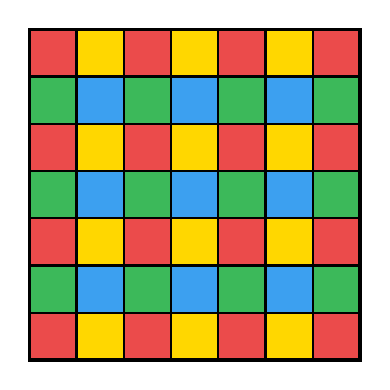
\begin{tikzpicture}[scale=0.6]
    \foreach \x in {0,...,6} {
        \foreach \y in {0,...,6} {
            \pgfmathsetmacro{\isYEven}{int(mod(\y, 2) == 0 ? 1 : 0)}
            \pgfmathsetmacro{\isXEven}{int(mod(\x, 2) == 0 ? 1 : 0)}
            \ifnum\isYEven=1
                \ifnum\isXEven=1
                    \fill[cellred] (\x, \y) rectangle ++(1, 1);
                \else
                    \fill[cellyellow] (\x, \y) rectangle ++(1, 1);
                \fi
            \else
                \ifnum\isXEven=1
                    \fill[cellgreen] (\x, \y) rectangle ++(1, 1);
                \else
                    \fill[cellblue] (\x, \y) rectangle ++(1, 1);
                \fi
            \fi
        }
    }
    \draw[draw=black, line width=0.8pt] (0, 0) grid (7, 7);
    \draw[draw=black, line width=1.2pt] (0, 0) rectangle (7, 7);
\end{tikzpicture}
\end{center}

খেয়াল কর, একটি খোঁড়া নৌকা একটি রুটে সবসময় নিচের ক্রমে (অথবা এর ঠিক বিপরীত ক্রমে) নির্দিষ্ট রঙের ঘরে যাতায়াত করে।
$$R, Y, B, G, R, Y, B, G, \ldots$$
তার মানে এমন একটি ক্রমের দৈর্ঘ্য $4T$, যেখানে $T$ হলো খোঁড়া নৌকাটির রুটে নীল রঙের ঘরের সংখ্যা।\\

এখন আমরা দেখাব যে, একটি খোঁড়া নৌকা কখনোই সবগুলো নীল রঙের ঘর দিয়ে যেতে পারবে না। ধর, খোঁড়া নৌকাটি সবগুলো নীল রঙের ঘর দিয়ে যেতে পারে। আমরা দুইটি নীল রঙের ঘরকে পরস্পর \textit{ক্রমিক} বলব যদি খোঁড়া নৌকাটি অন্য কোনো নীল রঙের ঘরকে অতিক্রম না করে একটি ঘর থেকে অপর ঘরে যাতায়াত করতে পারে। খেয়াল কর, দুটি ক্রমিক নীল রঙের ঘর হয় সোজাসুজি পাশাপাশি অবস্থান করে নতুবা কোণাকোণি পাশাপাশি অবস্থান করে।\\

দাবাবোর্ডের নীল রঙের ঘরগুলোকে পুনরায় সাদা-কালো রঙের বিন্যাসের অনুরূপ নেভি ব্লু-আসমানি রঙে রঙ করি। যেহেতু সর্বমোট বেজোড়সংখ্যক নীল রঙের ঘর রয়েছে, নেভি ব্লু এবং আসমানি রঙের ঘরের সংখ্যা পরস্পর অসমান। তার মানে কমপক্ষে একজোড়া কোণাকোণি পাশাপাশি অবস্থিত ক্রমিক নীল রঙের ঘর রয়েছে।\\

\begin{center}
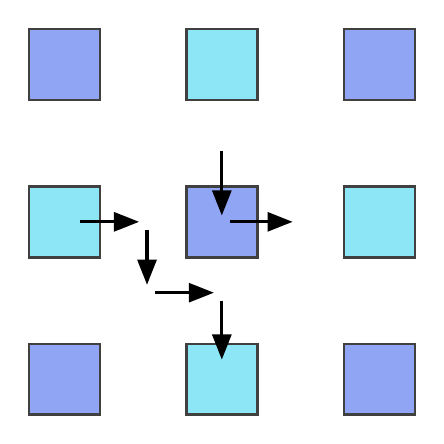
\begin{tikzpicture}[scale=1.0]
    \foreach \x in {0,1,2} {
        \foreach \y in {0,1,2} {
            \pgfmathsetmacro{\isEven}{int(mod(\x+\y, 2) == 0 ? 1 : 0)}
            \ifnum\isEven=1
                \fill[cellnavy] (2*\x-0.45, 2*\y-0.45) rectangle ++(0.9, 0.9);
                \draw[draw=black!75, line width=0.9pt] (2*\x-0.45, 2*\y-0.45) rectangle ++(0.9, 0.9);
            \else
                \fill[cellcyan] (2*\x-0.45, 2*\y-0.45) rectangle ++(0.9, 0.9);
                \draw[draw=black!75, line width=0.9pt] (2*\x-0.45, 2*\y-0.45) rectangle ++(0.9, 0.9);
            \fi
        }
    }

    \tikzset{
        myarrow/.style={-{Triangle[length=3.2mm, width=2.4mm]}, line width=1.2pt, draw=black}
    }

    \draw[myarrow] (0.2, 2.0) -- (0.95, 2.0);
    \draw[myarrow] (1.05, 1.9) -- (1.05, 1.2);
    \draw[myarrow] (1.15, 1.1) -- (1.9, 1.1);
    \draw[myarrow] (2.0, 1.0) -- (2.0, 0.25);

    \draw[myarrow] (2.0, 2.9) -- (2.0, 2.08);
    \draw[myarrow] (2.1, 2.0) -- (2.9, 2.0);
\end{tikzpicture}
\end{center}

\href{https://en.wikipedia.org/wiki/Without_loss_of_generality}{Without Loss of Generality}, খোঁড়া নৌকাটি নিচের মত করে চলাচল করে
$$(a,b+2) \to (a+1,b+2) \to (a+1,b+1) \to (a+2,b+1) \to (a+2,b).$$

যেহেতু খোঁড়া নৌকাটিকে $R, Y, B, G, \ldots$ এই ধারায় চলতে হবে, তাই একটা সময় খোঁড়া নৌকাটি $(a+2,b+3)\to(a+2,b+2)\to(a+3,b+2)$ এভাবে চলবে। তার মানে শেষমেশ খোঁড়া নৌকাটি $(a+2,b)$ থেকে $(a+2,b+3)$ এবং $(a+3,b+2)$ থেকে $(a,b+2)$ তে যাবে। এটা সহজেই বুঝা যাচ্ছে যে দুইটি পথ একে অপরকে ছেদ করবে, একটি কন্ট্রাডিকশন!\\

অর্থাৎ, একটি খোঁড়া নৌকার রুটের দৈর্ঘ্য সর্বোচ্চ $$4\left[\left(\frac{n-1}2\right)^2-1\right]=n^2-2n-3,$$ সমাধান শেষ!

\newpage

\section{অনুশীলনী}

\begin{flushleft}

\textbf{\textcolor{blue}{সমস্যা ১.} \textcolor{magenta}{(APMO 2007)}} একটি $5 \times 5$ বোর্ডের প্রতিটি ঘরে একটি করে লাইটবাল্ব রয়েছে। পুরো ব্যবস্থাটি ত্রুটিপূর্ণ, কারণ যেকোনো একটি বাল্বের সুইচ চাপলে শুধু ঐ বাল্বটিই না, এর ডানে, বামে, উপরে ও নিচের বাল্বেরও দশা পরিবর্তিত হয় (অর্থাৎ অফ থাকলে অন হয়, অন থাকলে অফ হয়)। শুরুতে সবগুলো লাইটবাল্ব অফ ছিল। কিছুসংখ্যক সুইচ চাপার পর ঠিক একটি বাল্ব জ্বলে রইল। জ্বলে থাকা বাল্বটির সম্ভাব্য সকল অবস্থান বের কর।

\textbf{\textcolor{blue}{সমস্যা ২.} \textcolor{magenta}{(USAMO 1998)}}
একটি কম্পিউটার স্ক্রিন $98 \times 98$ দাবাবোর্ড দেখায় (স্বাভাবিক সাদা-কালো বিন্যাসে রঙ করা)। ডিউক দাবাবোর্ডের লাইনের উপরে সবগুলো বাহু থাকে এমন যেকোনো আয়ত মাউস দিয়ে সিলেক্ট করতে পারে। যদি সে সিলেক্টেড আয়তের উপর মাউস দিয়ে ক্লিক করে, তাহলে ঐ আয়তের সবগুলো ঘরের রঙ পাল্টে যায় (কোনো ঘর সাদা হলে সেটা কালো হয়ে যায়, আবার কালো হলে সেটা সাদা হয়ে যায়)। সবচেয়ে কম কতবার মাউস ক্লিক করে সম্পূর্ণ বোর্ডটিকে একই রঙে রঙ করা যাবে?

\textbf{\textcolor{blue}{সমস্যা ৩.} \textcolor{magenta}{(Balkan 2000)}} সর্বোচ্চ কতগুলো $1 \times 10\sqrt{2}$ টাইল $50 \times 90$ আয়তের উপর বসানো যাবে, যেন কোনো ওভারল্যাপ না ঘটে এবং এমনভাবে বসানো হয় যাতে টাইলের বাহুগুলো আয়তের বাহুগুলোর সমান্তরালে থাকে?

\textbf{\textcolor{blue}{সমস্যা ৪.} \textcolor{magenta}{(ELMO 2021)}} একটি $100 \times 100$ বোর্ডে প্রতিটি ঘরকে $101$টি রঙের যেকোনো একটি দিয়ে রঙ করা হল। একটি ঘরকে \textit{বিচিত্র} বলা হবে, যদি এর সারি ও কলামের $199$টি ঘরগুলোর মধ্যে প্রতিটি রঙ অন্তত একবার থাকে। সম্ভাব্য সর্বোচ্চ বিচিত্র ঘরের সংখ্যা নির্ণয় কর।

\textbf{\textcolor{blue}{সমস্যা ৫.} \textcolor{magenta}{(IMO SL 2002)}} একটি বেজোড় ধনাত্মক পূর্ণসংখ্যা $n$ এর জন্য, একটি $n \times n$ দাবাবোর্ডের সবগুলো ঘর স্বাভাবিক সাদা-কালো রঙের বিন্যাসে রঙ করা যেন চারকোণার চারটি ঘর কালো হয়। $n$ এর কোন মানের জন্য দাবাবোর্ডটি L-ত্রিমিনো দিয়ে টাইল করা সম্ভব? যদি টাইল করা সম্ভব হয় তবে সর্বনিম্ন কতগুলো L-ত্রিমিনো লাগবে?

\textbf{\textcolor{blue}{সমস্যা ৬.} \textcolor{magenta}{(IMO SL 2000)}} একটি \textit{সিঁড়ি-ইট} হলো নিচের চিত্রের মতো $2$টি লেয়ারের $3$ ধাপবিশিষ্ট $12$টি ঘনক দিয়ে তৈরি একটি ইট যার প্রস্থ $2$ একক।

\begin{center}
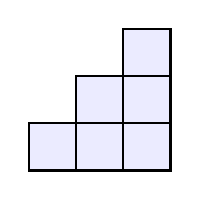
\begin{tikzpicture}[scale=0.6, line width=0.8pt]
    \foreach \x/\y in {0/0, 1/0, 1/1, 2/0, 2/1, 2/2} {
        \draw[fill=blue!8, draw=black] (\x, \y) rectangle ++(1, 1);
    }
\end{tikzpicture}
\end{center}

এমন সকল ধনাত্মক পূর্ণসংখ্যা $n$ বের কর যেন কিছুসংখ্যক সিঁড়ি-ইট দিয়ে $n$ একক বাহুবিশিষ্ট একটি ঘনক নির্মাণ করা সম্ভব।

\textbf{\textcolor{blue}{সমস্যা ৭.} \textcolor{magenta}{(IMO SL 2014)}}
দুইটি $2 \times 1$ ডমিনো তাদের লম্বা বাহুর সোজাসুজি যুক্ত করে একটি টেট্রামিনো গঠন করা হলো যেখানে একটি ডমিনোর একটি লম্বা বাহুর মধ্যবিন্দুটি অপর ডমিনোটির একটি কোণা। এভাবে দুইটি বিপরীত ওরিয়েন্টেশনে দুই ধরনের টেট্রামিনো গঠন করা সম্ভব। এদেরকে যথাক্রমে S-টেট্রামিনো এবং Z-টেট্রামিনো নাম দেওয়া হল। একটি \textit{ল্যাটিস বিন্দু} হলো সমতলের উপর এমন একটি বিন্দু যার ভুজ ও কোটি উভয়ই পূর্ণসংখ্যা। একটি বহুভুজের প্রতিটি শীর্ষবিন্দু একেকটি ল্যাটিস বিন্দু নির্দেশ করলে একে \textit{ল্যাটিস বহুভুজ} বলা হয়।

ধর একটি ল্যাটিস বহুভুজ $P$ কে S-টেট্রামিনো দ্বারা টাইল করা সম্ভব। প্রমাণ কর, $P$ কে S-টেট্রামিনো এবং Z-টেট্রামিনো দিয়ে যেভাবেই টাইল করা হোক না কেন, সবসময় জোড়সংখ্যক Z-টেট্রামিনো ব্যবহার করতে হবে।

\textbf{\textcolor{blue}{সমস্যা ৮.} \textcolor{magenta}{(IMO 2004)}}
একটি \textit{হুক} হলো নিচের চিত্রের মতো $6$টি বর্গাকার ঘর দিয়ে গঠিত একটি টাইল।

\begin{center}
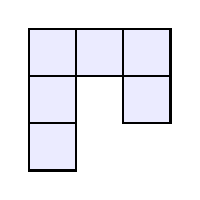
\begin{tikzpicture}[scale=0.6, line width=0.8pt]
    \foreach \x/\y in {0/0, 0/1, 0/2, 1/2, 2/2, 2/1} {
        \draw[fill=blue!8, draw=black] (\x, \y) rectangle ++(1, 1);
    }
\end{tikzpicture}
\end{center}

এমন সকল $m \times n$ আয়ত বের কর যেগুলো হুক দিয়ে টাইল করা সম্ভব।

\end{flushleft}

\begin{thebibliography}{9}

\bibitem{handout}
Yufei Zhao, \emph{\href{https://yufeizhao.com/olympiad/tiling.pdf}{Tiling: Coloring and Weights}}, MOP 2007

\bibitem{handout}
Matthew Brennan, \emph{\href{https://drive.google.com/file/d/1LKE1mfXuJ4U_5Ykbu5yErWba66G-7-BB/view}{Grids and Related Problems}}, Canadian IMO Training 2018

\bibitem{book}
Arthur Engel, \emph{\href{https://mathematicalolympiads.files.wordpress.com/2012/08/75427434-problem-books-in-mathematics-problem-solving-strategies.pdf}{Problem-Solving Strategies}}

\bibitem{book}
Pranav A. Sriram, \emph{\href{https://cdn.bc-pf.org/resources/math/combinatorics/Pranav_Sriram-Olympiad_Combinatorics.pdf}{Olympiad Combinatorics}}

\bibitem{website}
Bangladesh Mathematical Olympiad, \emph{\href{https://matholympiad.org.bd/questions}{BdMO Problems}}

\bibitem{website}
Art of Problem Solving, \emph{\href{https://artofproblemsolving.com/}{AoPS}}

\end{thebibliography}

\end{document}
